\documentclass{templateNote}
\usepackage{tcolorbox}
\usepackage{pgfplots}
\usepackage{pgf-pie}
\usepackage{tabularx}
\usepackage{graphicx}
\usepackage{tikz}

\newcolumntype{L}{>{\centering\arraybackslash}X}
\pgfmathdeclarefunction{gauss}{2}{%
  \pgfmathparse{1/(#2*sqrt(2*pi))*exp(-((x-#1)^2)/(2*#2^2))}%
}
\begin{document}

\imagenlogo{img/logoUBB.png}
\universidad{Universidad del Bío-Bío pepito5}
\titulo{Estadistica Descriptiva} % Titulo
\asignatura{Estadistica y Probabilidades} % Asignatura
\autor{
    \indent
    Marcelo \textsc{Paz}
}   
\portada
\margenes % Crear márgenes

\section{Definiciones generales}
\begin{enumerate}
    \item \textbf{Estadística:} Ciencia que estudia los métodos para recoger, organizar, resumir y analizar datos, así como para sacar conclusiones válidas y tomar decisiones razonables basadas en tal análisis.\\
    \item \textbf{Estadística Descriptiva:} Parte de la estadística que se ocupa de la recolección, presentación, descripción, análisis y resumen de datos.\\
\end{enumerate}
\section{Tipos de variables}
\begin{enumerate}
    \item \textbf{Variable cualitativa:} Es aquella que no se puede medir numéricamente, sino que se clasifica en categorías.\\
    \item \textbf{Variable cuantitativa:} Es aquella que se puede medir numéricamente.\\
    \begin{enumerate}
        \item \textbf{Variable discreta:} Es aquella que puede tomar valores aislados, es decir, no puede tomar todos los valores posibles entre dos valores cualesquiera.\\
        \item \textbf{Variable continua:} Es aquella que puede tomar todos los valores posibles entre dos valores cualesquiera.\\
    \end{enumerate}
\end{enumerate}

\newpage
\section{Graficos}
\subsection{Tabla de frecuencias:}
\indent
Es una tabla que representa los datos de forma ordenada en columnas.\\
\begin{figure}[H]
    \centering
    \begin{tabularx}{\textwidth}{|L|L|L|L|}
        \hline
        \textbf{Signos Visibles} & \textbf{Frecuencia Absoluta $f_i$} & \textbf{Frecuencia Acumulada $F_i$} & \textbf{Frecuencia relativa porcentual $fr_i$} \\
        \hline
        Dieta Severa & 9 & 9 & 33\% \\
        \hline
        Uso de Ropa Holgada & 6 & 15 & 22\% \\
        \hline
        Miedo a Engordar & 3 & 18 & 11\% \\
        \hline
        Hiperactividad & 4 & 22 & 15\% \\
        \hline
        Uso de Laxantes & 5 & 27 & 19\% \\
        \hline
        Total & 27 & & 100\% \\
        \hline
    \end{tabularx}
    \caption{Tabla de frecuencias de datos \textbf{cualitativos}}
\end{figure}

\begin{figure}[H]
    \centering
    \begin{tabularx}{\textwidth}{|L|L|L|L|}
        \hline
        \textbf{Número de asignaturas reprobadas $c_i$} & \textbf{Frecuencia Absoluta $f_i$} & \textbf{Frecuencia Acumulada $F_i$} & \textbf{Frecuencia Relativa porcentual $fr_i$} \\
        \hline
        0 & 26 & 26 & 28,8\% \\
        1 & 17 & 43 & 18,8\% \\
        2 & 21 & 64 & 23,3\% \\
        3 & 11 & 75 & 12,2\% \\
        4 & 7 & 82 & 7,7\% \\
        5 & 4 & 86 & 4,4\% \\
        6 & 3 & 89 & 3,3\% \\
        7 & 1 & 90 & 1,1\% \\
        \hline
        Total & 90 & & 100\% \\
        \hline
    \end{tabularx}
    \caption{Tabla de frecuencias de datos \textbf{cuantitativos discretos}}
\end{figure}

\begin{figure}[H]
    \centering
    \begin{tabularx}{\textwidth}{|L|L|L|L|L|}
        \hline
        \textbf{Fronteras} & \textbf{Frecuencia Absoluta $f_i$} & \textbf{Frecuencia Acumulada $F_i$} & \textbf{Frecuencia relativa porcentual $fr_i$} & \textbf{Marca de clase $m_i$} \\
        \hline
        1,5 - 2,5 & 5 & 5 & 10\% & 2 \\
        2,5 - 3,5 & 14 & 19 & 28\% & 3 \\
        3,5 - 4,5 & 6 & 25 & 12\% & 4 \\
        4,5 - 5,5 & 25 & 50 & 50\% & 5 \\
        \hline
        Total & 50 & & 100\% &  \\
        \hline
    \end{tabularx}
    \caption{Tabla de frecuencias de datos \textbf{cuantitativos continuos}}
\end{figure}

\newpage
\subsection{Histograma:}
\indent
Es un gráfico de barras. Se construye ubicando en el eje horizontal a las fronteras y en el
vertical a las frecuencias absolutas. Su particularidad es que las barras están pegadas,
pues comparten un lado en común. Su utilidad se aprecia cuando se quiere estudiar la
forma de la distribución. Esto es, cuando se quiere estudiar la simetría o sesgo de los datos

\begin{figure}[H]
    \centering
    \begin{tikzpicture}
        \begin{axis}[
            xtick distance=1,
            ytick distance=2,
            width = 17cm,
            ymin = 0,
            height = 8cm,
            xlabel={Número de asignaturas reprobadas $c_i$},
            ylabel={$f_i$}
        ]
        \addplot+[ycomb] plot coordinates
        {(0,26) (1,17) (2,21) (3,11) (4,7) (5,4) (6,3) (7,1)};
        \end{axis}
    \end{tikzpicture}
    \caption{Histograma de datos \textbf{cuantitativos discretos}}
\end{figure}

\begin{figure}[H]
    \centering
    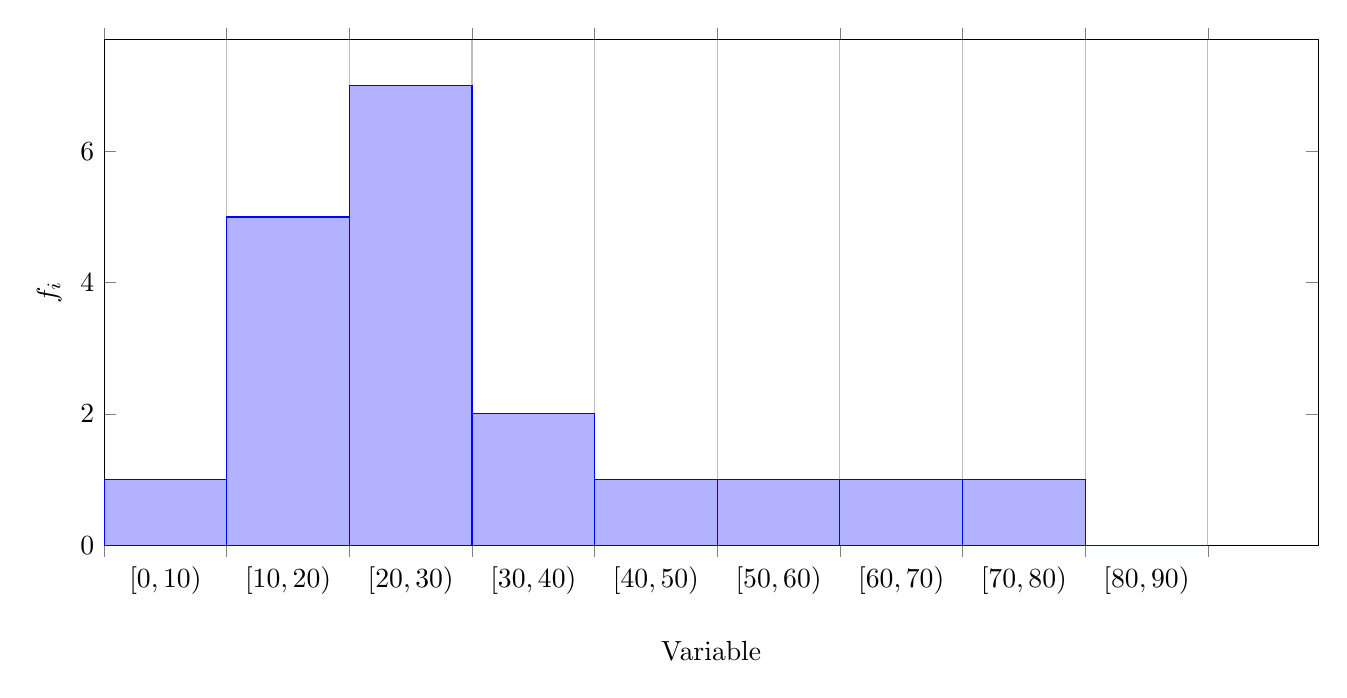
\begin{tikzpicture}
        \begin{axis}[
            ybar interval,
            xlabel = {Variable},
            ylabel = \(f_i\),
            xlabel style = {yshift=-1em},
            width = 17cm,
            xmin = 0,
            ymin = 0,
            height = 8cm,
            xticklabel=
            {$[\pgfmathprintnumber\tick,%
                \pgfmathprintnumber\nexttick)$}
        ]
            \addplot coordinates {
                (0, 1) (10, 5)
                (20, 7) (30, 2)
                (40, 1) (50, 1)
                (60, 1) (70, 1)
                (80, 0) (90, 1)
            };
        \end{axis}
    \end{tikzpicture}
    \caption{Histograma de datos \textbf{cuantitativos continuos}}
\end{figure}

\newpage
\subsection{Polígono de frecuencia:}
\indent
Es un gráfico que consiste en destacar las marcas de clase de cada intervalo frente a sus
correspondientes frecuencias absolutas. Cada marca de clase se une con segmentos de
rectas que generan la curva. Para cerrar el área se utilizan las marcas de clase ficticias: La
primera se crea restando la amplitud a la marca de clase del primer intervalo y la segunda
se crea sumando la amplitud a la marca de clase del último intervalo. Su utilidad se aprecia
cuando se quiere comprar dos o más distribuciones de frecuencias. Generalmente se dibuja
sobre el Histograma.
\begin{figure}[H]
    \centering
    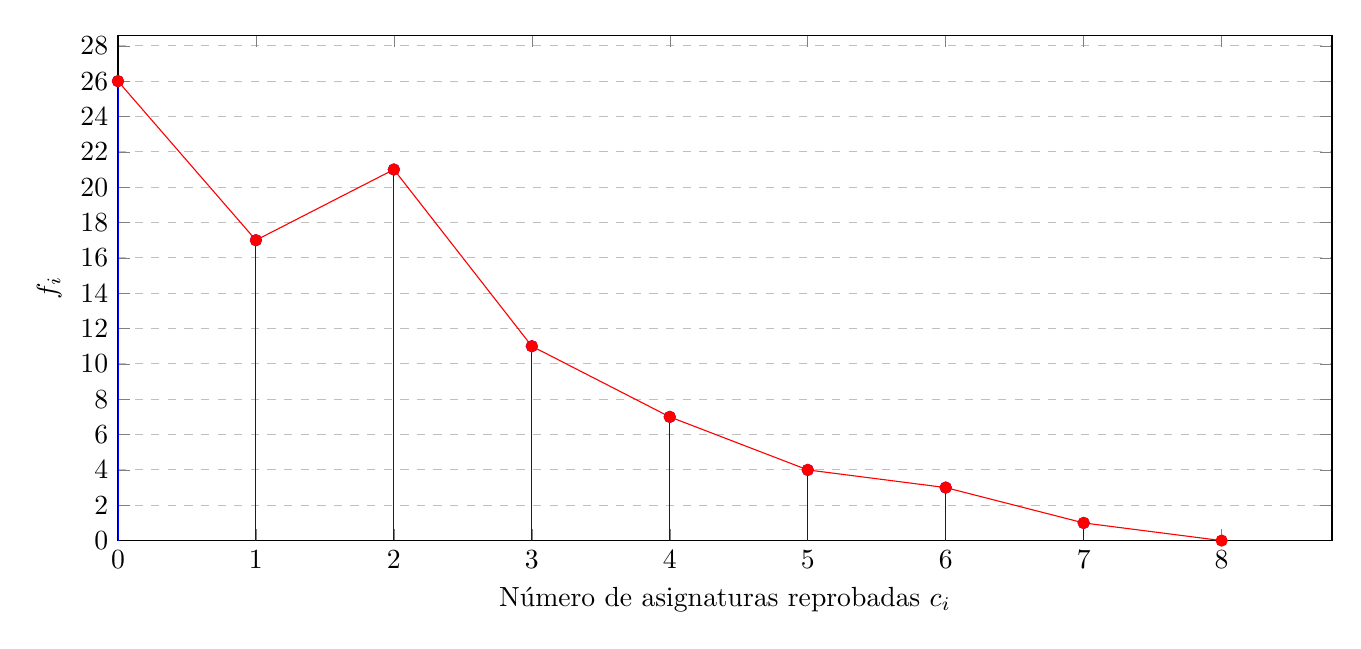
\begin{tikzpicture}
        \begin{axis}[
            xtick distance=1,
            ytick distance=2,
            ymajorgrids=true,
            grid style=dashed,
            width = 17cm,
            xmin = 0,
            ymin = 0,
            height = 8cm,
            xlabel={Número de asignaturas reprobadas $c_i$},
            ylabel={$f_i$}
        ]
        \addplot+[ycomb] plot coordinates
        {(0,26) (1,17) (2,21) (3,11) (4,7) (5,4) (6,3) (7,1)};
        \addplot[color=red,mark=*] coordinates {(0,26) (1,17) (2,21) (3,11) (4,7) (5,4) (6,3) (7,1) (8,0)};
        \end{axis}
    \end{tikzpicture}
    \caption{Histograma y Poligono de frecuencias de datos \textbf{cuantitativos discretos}}
\end{figure}

\begin{figure}[H]
    \centering
    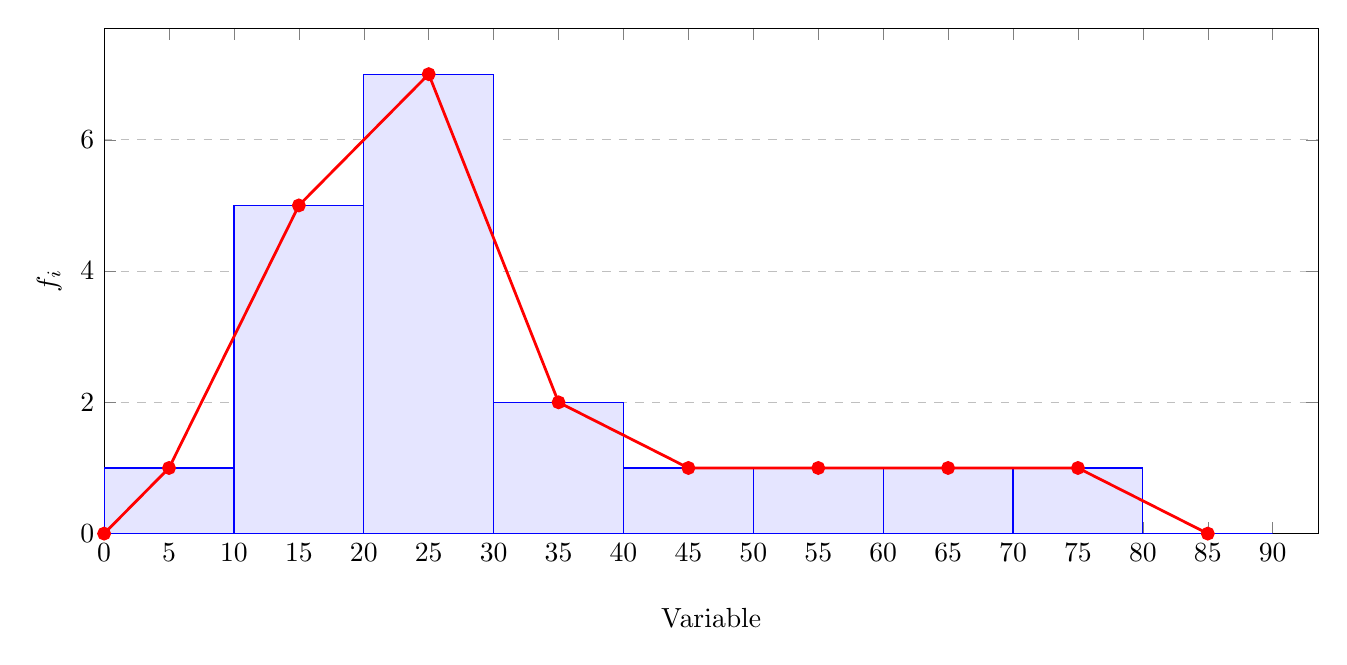
\begin{tikzpicture}
        \begin{axis}[
            xlabel = {Variable},
            ylabel = \(f_i\),
            xlabel style = {yshift=-1em},
            xmin = 0,
            xtick distance=5,
            ymin = 0,
            ymajorgrids=true,
            grid style=dashed,
            width = 17cm,
            height = 8cm,
        ]
            \draw [blue, fill= blue!10] (axis cs:0,0) rectangle (axis cs:10,1);
            \draw [blue, fill= blue!10] (axis cs:10,0) rectangle (axis cs:20,5);
            \draw [blue, fill= blue!10] (axis cs:20,0) rectangle (axis cs:30,7);
            \draw [blue, fill= blue!10] (axis cs:30,0) rectangle (axis cs:40,2);
            \draw [blue, fill= blue!10] (axis cs:40,0) rectangle (axis cs:50,1);
            \draw [blue, fill= blue!10] (axis cs:50,0) rectangle (axis cs:60,1);
            \draw [blue, fill= blue!10] (axis cs:60,0) rectangle (axis cs:70,1);
            \draw [blue, fill= blue!10] (axis cs:70,0) rectangle (axis cs:80,1);
            \draw [blue, fill= blue!10] (axis cs:80,0) rectangle (axis cs:90,0);
            \addplot[color=red,mark=*, line width=1pt] coordinates {
                (0,0)
                (5,1)
                (15,5)
                (25,7)
                (35,2)
                (45,1)
                (55,1)
                (65,1)
                (75,1)
                (85,0)
            };
        \end{axis}
    \end{tikzpicture}
    \caption{Histograma y Poligono de frecuencia de datos \textbf{cuantitativos continuos}}
\end{figure}

\newpage
\subsection{Ojiva:}
\indent
Es un gráfico de frecuencia acumulada. Se gráfica única y exclusivamente con las fronteras
en el eje horizontal. Su utilidad se aprecia cuando se cuenta con medidas de posición tales
como: Cuartiles, Deciles y Percentiles.
\begin{figure}[H]
    \centering
    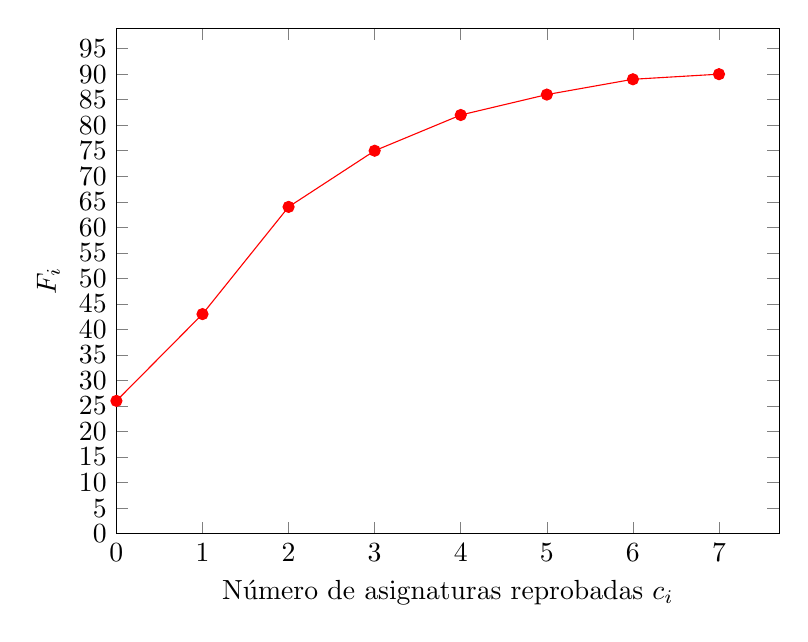
\begin{tikzpicture}
        \begin{axis}[
            xtick distance=1,
            ytick distance=5,
            width = 10cm,
            xmin = 0,
            ymin = 0,
            height = 8cm,
            xlabel={Número de asignaturas reprobadas $c_i$},
            ylabel={$F_i$}
        ]
        \addplot[color=red,mark=*] coordinates {(0,26) (1,43) (2,64) (3,75) (4,82) (5,86) (6,89) (7,90)};
        \end{axis}
    \end{tikzpicture}
    \caption{Ojiva de datos \textbf{cuantitativos discretos}}
\end{figure}

\begin{figure}[H]
    \centering
    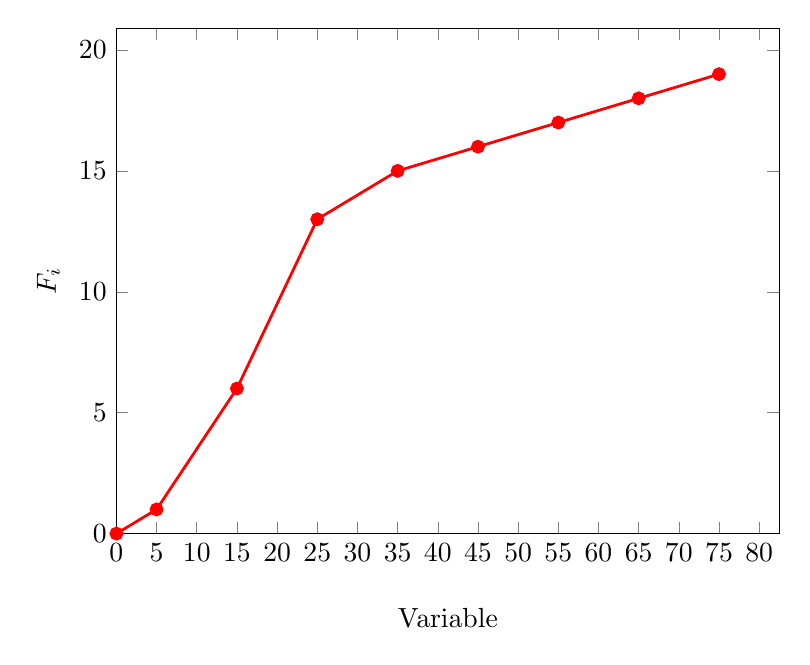
\begin{tikzpicture}
        \begin{axis}[
            xlabel = {Variable},
            ylabel = \(F_i\),
            xlabel style = {yshift=-1em},
            xmin = 0,
            xtick distance=5,
            ymin = 0,
            width = 10cm,
            height = 8cm,
        ]
            \addplot[color=red,mark=*, line width=1pt] coordinates {
                (0,0)
                (5,1)
                (15,6)
                (25,13)
                (35,15)
                (45,16)
                (55,17)
                (65,18)
                (75,19)
            };
        \end{axis}
    \end{tikzpicture}
    \caption{Ojiva de datos \textbf{cuantitativos continuos}}
\end{figure}

\newpage
\section{Medidas de tendencia central}
\subsection{Media aritmética:}
Es la suma de todos los datos dividida por el total. Cambia un poco en su forma según como
estén presentados los datos.
\begin{enumerate}
    \item \textbf{Datos no agrupados:}
    \begin{equation*}
        \overline{x} = \frac{\displaystyle \sum_{i=1}^{n} x_i}{n}
    \end{equation*}
    * $x_i$ es cada dato.
    \item \textbf{Datos agrupados(discreta):}
    \begin{equation*}
        \overline{x} = \frac{\displaystyle \sum_{i=1}^{k} f_i \cdot c_i}{n}
    \end{equation*}
    * $c_i$ es cada dato.
    \item \textbf{Datos agrupados(continua):}
    \begin{equation*}
        \overline{x} = \frac{\displaystyle \sum_{i=1}^{k} f_i \cdot m_i}{n}
    \end{equation*}
    * $m_i$ es la marca de clase de cada dato.
\end{enumerate}
* $f_i$ es la frecuencia absoluta de cada dato.\\
* $n$ es el total de datos.\\
* $k$ es el total de intervalos.

\subsection{Mediana:}
Es el valor que ocupa la posición central en un conjunto de datos ordenados. Cambia un
poco en su forma según como estén presentados los datos.
\begin{enumerate}
    \item \textbf{Datos no agrupados:} es necesario ordenar de menor a mayor los datos.
    \begin{equation*}
        M_e = \displaystyle \left\{ \begin{array}{ll}
            x_{\frac{n+1}{2}} & \textrm{si $n$ es impar}\\
            \frac{\displaystyle x_{\frac{n}{2}} + x_{\frac{n}{2}+1}}{2} & \textrm{si $n$ es par}
        \end{array} \right.
    \end{equation*}
    \item \textbf{Datos agrupados(discreta):}
    $M_e$ Es el valor de la clase o categoria ($c_i$) donde se encuentra la mitad de los datos en la columna de la frecuencia acumulada.
    \newpage
    \item \textbf{Datos agrupados(continua):}
    \begin{equation*}
        M_e = FI_k + \left(\frac{\displaystyle \frac{n}{2} - F_{k-1}}{f_k}\right) \cdot A_k
    \end{equation*}
\end{enumerate}
* $FI_k$ es la Frontera Inferior de la clase mediana.\\
* $FI_k$ es la frecuencia absoluta acumulada de la clase anterior a la clase mediana.\\
* $f_k$ es la frecuencia absoluta de la clase.\\
* $A_k$ es la amplitud de la clase mediana.\\
* $n$ es el total de datos.\\
\subsection{Moda:}
Es el valor que más se repite en un conjunto de datos. Cambia un poco en su forma según
como estén presentados los datos.
\begin{enumerate}
    \item \textbf{Datos no agrupados:} es necesario ordenar de menor a mayor los datos.
    \begin{equation*}
        M_o = \textrm{Valor que más se repite}
    \end{equation*}
    \item \textbf{Datos agrupados(discreta):}
    $M_o$ Es el valor de la clase o categoria ($c_i$) donde se encuentra la mayor frecuencia absoluta.
    \item \textbf{Datos agrupados(continua):}
    \begin{equation*}
        M_o = FI_k + \left(\frac{a}{a + b}\right) \cdot A_k
    \end{equation*}
\end{enumerate}
* $FI_k$ es la Frontera Inferior de la clase modal.\\
* $a$ es la Diferencia entre la frecuencia absoluta de la clase modal y la frecuencia absoluta de la clase anterior a la clase modal.\\
* $b$ es la Diferencia entre la frecuencia absoluta de la clase modal y la frecuencia absoluta de la clase posterior a la clase modal.\\
* $A_k$ es la amplitud de la clase modal.\\

\subsection{Resumen}
\begin{figure}[H]
    \centering
    \begin{tabularx}{\textwidth}{|L|L|L|L|}
        \hline
        \textbf{Descripción} & \textbf{Media $\overline{x}$} & \textbf{Mediana $M_e$} & \textbf{Moda $M_o$} \\
        \hline
        \textbf{Datos NO agrupados} & 
        \[
            \overline{x} = \frac{\displaystyle \sum_{i=1}^{n} x_i}{n}
        \] & Si el total de observaciones es impar, la mediana es el valor que se encuentra justo en la mitad del conjunto previamente ordenado de menor a mayor. Si el total de observaciones es par, la mediana es el promedio de las dos observaciones centrales del conjunto previamente ordenado. &
        Valor que más se repite. \textbf{Unimodal:} una moda. \textbf{Bimodal:} dos modas. \textbf{Multimodal:} mas de 2 modas\\
        \hline
        \textbf{Datos agrupados (discreta)} & 
        \[
            \overline{x} = \frac{\displaystyle \sum_{i=1}^{n} f_i c_i}{n}
        \] & Es el valor de la clase o categoria ($c_i$) donde se encuentra la mitad de los datos en la columna de la frecuencia acumulada. &
        Es el valor de la clase o categoria ($c_i$) donde se encuentra la frecuencia absoluta mas alta.\\
        \hline
        \textbf{Datos agrupados (continua)} & 
        \[
            \overline{x} = \frac{\displaystyle \sum_{i=1}^{n} f_i m_i}{n}
        \] &
        \begin{equation*}
            \scalebox{0.6}{$M_e = FI_k + \left(\frac{\displaystyle \frac{n}{2} - F_{k-1}}{f_k}\right) \cdot A_k$}   
        \end{equation*}
        &
        \begin{equation*}
            \scalebox{0.8}{$M_o = FI_k + \left(\frac{a}{a+b}\right) \cdot A_k$}
        \end{equation*} \\
        \hline
    \end{tabularx}
    \caption{Tabla Resumen \textbf{Medidas de Tendencia Central}}
\end{figure}

\newpage
\section{Medidas de dispersión}
\indent
Nos indican que tanto se alejan los datos del centro. Las más utilizadas en Estadística
Descriptiva son:
\subsection{Varianza}
\indent
Es el promedio cuadrado de las distancias
entre cada observación y el promedio de ellos.
Se denota por $S^2$
. Su gran desventaja es que
crece conforme crecen los datos y también
puede ser cero si estos, son muy parecidos
entre si.

Se utiliza la media $\overline{x}$
\begin{enumerate}
    \item \textbf{Datos no agrupados:}
    \begin{equation*}
        s^2 = \frac{\displaystyle \sum_{i=1}^{n} (x_i - \overline{x})^2}{n}
    \end{equation*}
    * $x_i$ es cada dato.\\
    \item \textbf{Datos agrupados (discreta):}
    \begin{equation*}
        s^2 = \frac{\displaystyle \sum_{i=1}^{n} (c_i - \overline{x})^2 f_i}{n}
    \end{equation*}
    * $c_i$ es cada dato.\\
    \item \textbf{Datos agrupados (continua):}
    \begin{equation*}
        s^2 = \frac{\displaystyle \sum_{i=1}^{n} (m_i - \overline{x})^2 f_i}{n}
    \end{equation*}
    * $m_i$ es la marca de clase de cada dato.
\end{enumerate}
* $f_i$ es la frecuencia absoluta de cada dato.\\
* $n$ es el total de datos.\\

\subsection{Desviación Estandar}
\indent
Es la raíz cuadrada de la varianza. Su gran
ventaja por sobre ésta, es que entrega sus
resultados en la misma unidad de medida que
la variable.
\begin{equation*}
    s = \sqrt{s^2}
\end{equation*}
* $s^2$ es la varianza.\\

\subsection{Coeficiente de Variación}
\indent
Se define como el cuociente entre la
desviación estándar y el promedio de los datos.
Generalmente se entrega en porcentaje. Su
gran ventaja es que sus resultados carecen de
unidad de medida, por lo que permite comparar
datos aunque estén en distinta unidades de
medida.
\begin{equation*}
    CV = \frac{s}{\overline{x}} \cdot 100
\end{equation*}
* $s$ es la desviación estándar.\\
* $\overline{x}$ es la media.\\

\subsection{Rango}
\indent
Es la diferencia entre el máximo y el mínimo de
los datos. Su utilidad se aprecia cuando
tenemos más información de la variable. 
\begin{equation*}
    R = x_{max} - x_{min}
\end{equation*}
* $x_{max}$ es el valor máximo de los datos.\\
* $x_{min}$ es el valor mínimo de los datos.\\

\section{Medidas de posición}
\indent
Son aquellas que permiten conocer con mayor detalle a una variable. Entre se encuentran
los:
\subsection{Cuartiles}
Dividen al conjunto de datos en cuatro partes porcentualmente iguales.
\[
    Q_k \quad \text{, k = 1,2,3} \quad
    \text{, donde: } Q_1 = 25\% \quad Q_2 = 50\% \quad Q_3 = 75\%
\]
\begin{enumerate}
    \item Para datos cuantitativos discretos:
    \begin{equation*}
        Q_k = \frac{kn}{4}
    \end{equation*}
    \item Para datos cuantitativos continuos:
    \begin{equation*}
        Q_k = FI_k + \left(\frac{\displaystyle \frac{kn}{4} - F_{k-1}}{f_k}\right) \cdot A_k
    \end{equation*}
    * $FI_k$ es la Frontera Inferior de la clase del k-esimo cuartil.\\
    * $F_{k-1}$ es la frecuencia acumulada hasta la clase anterior a la clase del k-esimo cuartil. \\
    * $f_k$ es la frecuencia absoluta de la clase del k-esimo cuartil.\\
    * $A_k$ es la amplitud de la clase del k-esimo cuartil.\\
\end{enumerate}

\newpage
\subsection{Deciles}
Dividen al conjunto de datos en diez partes porcentualmente iguales.
\[
    D_k \quad \text{, k = 1,2,...,8,9} \quad
    \text{, donde: } D_1 = 10\% \quad ...\quad D_9 = 90\%
\]
\begin{enumerate}
    \item Para datos cuantitativos discretos:
    \begin{equation*}
        D_k = \frac{kn}{10}
    \end{equation*}
    \item Para datos cuantitativos continuos:
    \begin{equation*}
        D_k = FI_k + \left(\frac{\displaystyle \frac{kn}{10} - F_{k-1}}{f_k}\right) \cdot A_k
    \end{equation*}
    * $FI_k$ es la Frontera Inferior de la clase del k-esimo decil.\\
    * $F_{k-1}$ es la frecuencia acumulada hasta la clase anterior a la clase del k-esimo decil. \\
    * $f_k$ es la frecuencia absoluta de la clase del k-esimo decil.\\
    * $A_k$ es la amplitud de la clase del k-esimo decil.\\
\end{enumerate}

\subsection{Percentiles}
Dividen al conjunto de datos en cien partes porcentualmente iguales.
\[
    P_k \quad \text{, k = 1,2,...,98,99} \quad
    \text{, donde: } P_1 = 1\% \quad ...\quad P_{99} = 99\%
\]
\begin{enumerate}
    \item Para datos cuantitativos discretos:
    \begin{equation*}
        D_k = \frac{kn}{10}
    \end{equation*}
    \item Para datos cuantitativos continuos:
    \begin{equation*}
        D_k = FI_k + \left(\frac{\displaystyle \frac{kn}{10} - F_{k-1}}{f_k}\right) \cdot A_k
    \end{equation*}
    * $FI_k$ es la Frontera Inferior de la clase del k-esimo percentil.\\
    * $F_{k-1}$ es la frecuencia acumulada hasta la clase anterior a la clase del k-esimo percentil. \\
    * $f_k$ es la frecuencia absoluta de la clase del k-esimo percentil.\\
    * $A_k$ es la amplitud de la clase del k-esimo percentil.\\
\end{enumerate}

\newpage
\section{Simetría}
\begin{equation*}
    f_1 = f_k \quad f_2 = f_{k-1} \quad f_3 = f_{k-2} \quad \text{... etc}
\end{equation*}

\subsection{Unimodal}
\begin{equation*}
    \overline{x} = M_e = M_o
\end{equation*}

\begin{figure}[H]
    \centering
    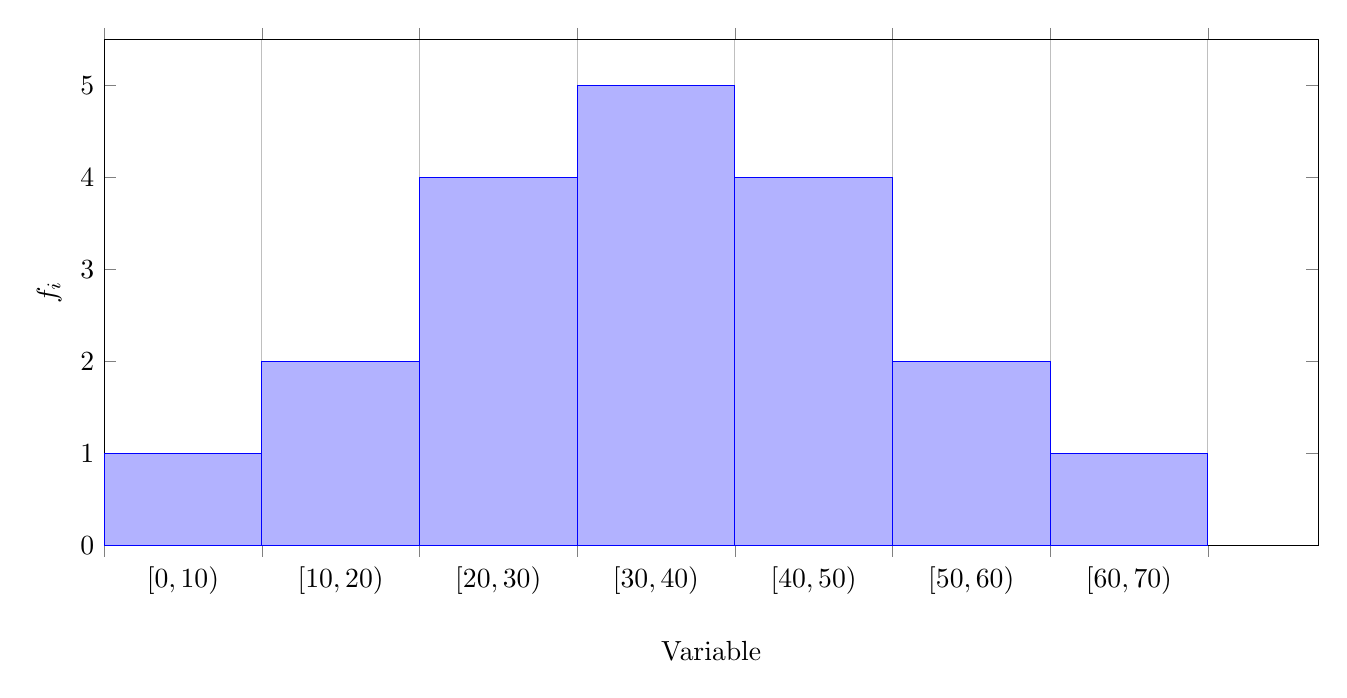
\begin{tikzpicture}
        \begin{axis}[
            ybar interval,
            xlabel = {Variable},
            ylabel = \(f_i\),
            xlabel style = {yshift=-1em},
            width = 17cm,
            ymin = 0,
            xmin = 0,
            height = 8cm,
            xticklabel=
            {$[\pgfmathprintnumber\tick,%
                \pgfmathprintnumber\nexttick)$}
        ]
            \addplot coordinates {
                (0, 1) (10, 2)
                (20, 4) (30, 5)
                (40, 4) (50, 2)
                (60, 1) (70, 1)
            };
        \end{axis}
    \end{tikzpicture}
    \caption{Distribución \textbf{simétrica y unimodal}}
\end{figure}

\subsection{Bimodal}

\begin{figure}[H]
    \centering
    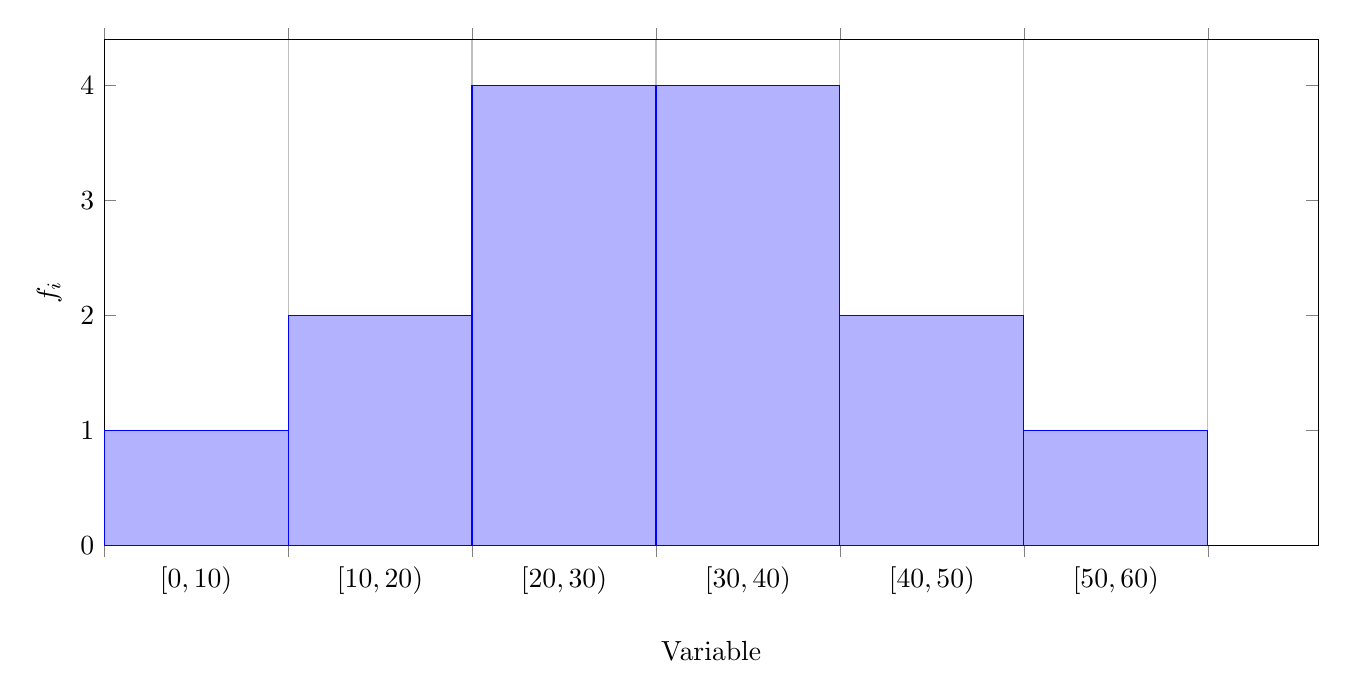
\begin{tikzpicture}
        \begin{axis}[
            ybar interval,
            xlabel = {Variable},
            ylabel = \(f_i\),
            xlabel style = {yshift=-1em},
            width = 17cm,
            ymin = 0,
            xmin = 0,
            height = 8cm,
            xticklabel=
            {$[\pgfmathprintnumber\tick,%
                \pgfmathprintnumber\nexttick)$}
        ]
            \addplot coordinates {
                (0, 1) (10, 2)
                (20, 4) (30, 4)
                (40, 2) (50, 1)
                (60, 1)
            };
        \end{axis}
    \end{tikzpicture}
    \caption{Distribución \textbf{simétrica y bimodal en el centro}}
\end{figure}
\begin{figure}[H]
    \centering
    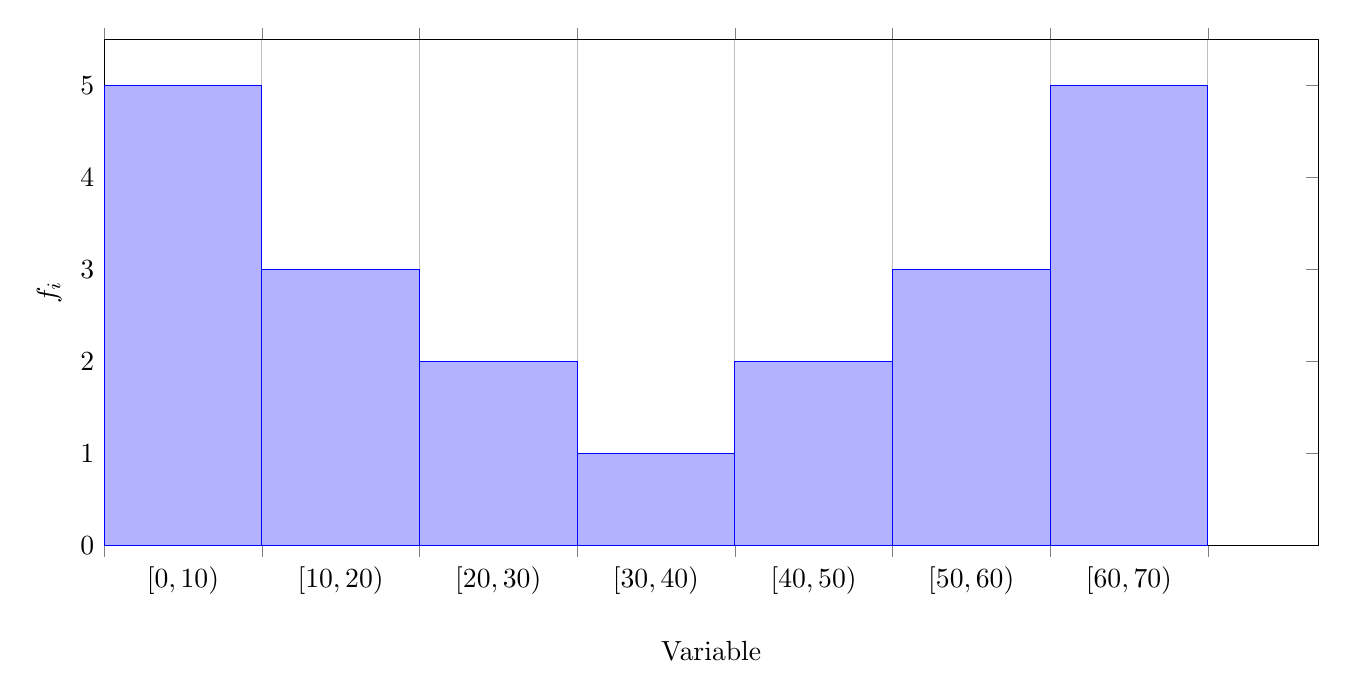
\begin{tikzpicture}
        \begin{axis}[
            ybar interval,
            xlabel = {Variable},
            ylabel = \(f_i\),
            xlabel style = {yshift=-1em},
            width = 17cm,
            ymin = 0,
            xmin = 0,
            height = 8cm,
            xticklabel=
            {$[\pgfmathprintnumber\tick,%
                \pgfmathprintnumber\nexttick)$}
        ]
            \addplot coordinates {
                (0, 5) (10, 3)
                (20, 2) (30, 1)
                (40, 2) (50, 3)
                (60, 5) (70, 5)
            };
        \end{axis}
    \end{tikzpicture}
    \caption{Distribución \textbf{simétrica y bimodal en los extremos}}
\end{figure}

\section{Sesgo (Asimétria)}
\indent
El sesgo es un comportamiento que se da en las medidas de tendencia central y es de la
siguiente forma:
\subsection{Positivo o a la derecha}
\begin{equation*}
    \overline{x} > M_e > M_o
\end{equation*}
\begin{figure}[H]
    \centering
    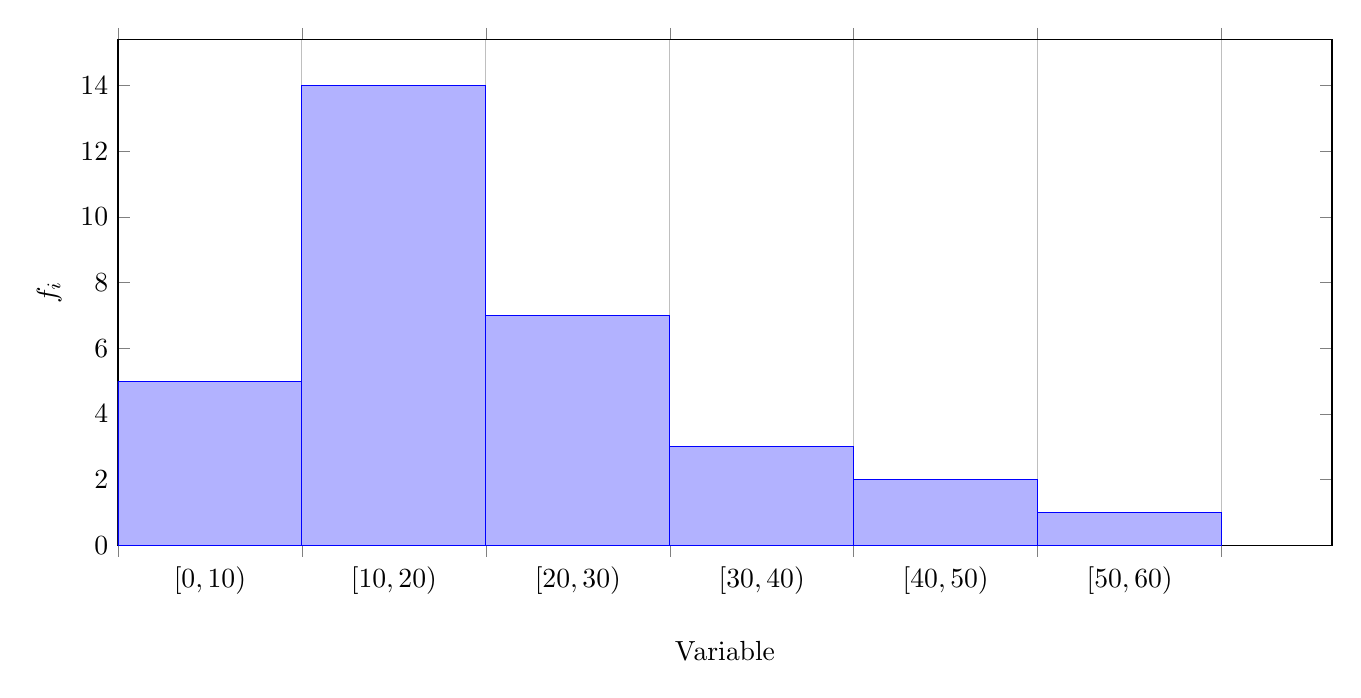
\begin{tikzpicture}
        \begin{axis}[
            ybar interval,
            xlabel = {Variable},
            ylabel = \(f_i\),
            xlabel style = {yshift=-1em},
            width = 17cm,
            ymin = 0,
            xmin = 0,
            height = 8cm,
            xticklabel=
            {$[\pgfmathprintnumber\tick,%
                \pgfmathprintnumber\nexttick)$}
        ]
            \addplot coordinates {
                (0, 5) (10, 14)
                (20, 7) (30, 3)
                (40, 2) (50, 1)
                (60, 1)
            };
        \end{axis}
    \end{tikzpicture}
    \caption{Distribución \textbf{asimétrica positiva}}
\end{figure}

\subsection{Negativo o a la izquierda}
\begin{equation*}
    \overline{x} < M_e < M_o
\end{equation*}
\begin{figure}[H]
    \centering
    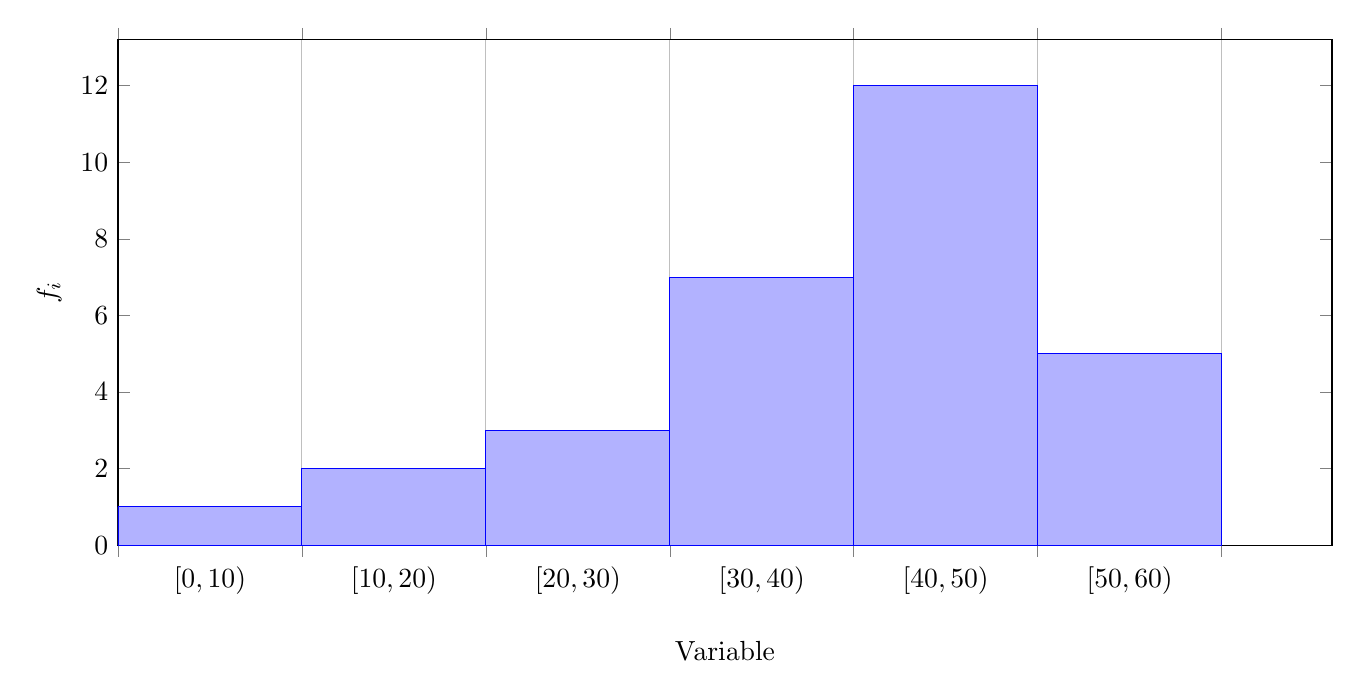
\begin{tikzpicture}
        \begin{axis}[
            ybar interval,
            xlabel = {Variable},
            ylabel = \(f_i\),
            xlabel style = {yshift=-1em},
            width = 17cm,
            ymin = 0,
            xmin = 0,
            height = 8cm,
            xticklabel=
            {$[\pgfmathprintnumber\tick,%
                \pgfmathprintnumber\nexttick)$}
        ]
            \addplot coordinates {
                (0, 1) (10, 2)
                (20, 3) (30, 7)
                (40, 12) (50, 5)
                (60, 5)
            };
        \end{axis}
    \end{tikzpicture}
    \caption{Distribución \textbf{asimétrica positiva}}
\end{figure}

\subsection{Coeficientes de asimétria}
\begin{equation*}
    CA_1 = \frac{\overline{x} - M_o}{s} \\
    CA_2 = \frac{3(\overline{x} - M_e)}{s} \\
    CA_3 = \frac{Q_1 - 2Q_2 + Q_3}{Q_3 - Q_1} \\
\end{equation*}
* donde $Q_3 - Q_1$ se conoce como rango intercuartílico. \\
* $CA_1 \ne CA_2 \ne CA_3$, pero coiciden en signo.\\
\begin{enumerate}
    \item Si el \textbf{coeficiente es positivo}: se dice que la asimetría es positiva y el sesgo va a la derecha.
    \item Si el \textbf{coeficiente es negativo}: se dice que la asimetría es negativo y el sesgo va a la izquierda.
\end{enumerate}

\section{Regla Empírica}
\indent
Si una distribución es simétrica, unimodal de forma acampanada, se dice \textbf{Aproximadamente Normal}

\begin{figure}[H]
    \centering
    \begin{tikzpicture}
        \begin{axis}[
            no markers, 
            domain=-4:4, 
            samples=100,
            xtick={-3,-2,-1,0,1,2,3},
            xticklabels={$\overline{x} - 3s$, $\overline{x} - 2s$, $\overline{x} - s$, $\overline{x}$, $\overline{x} + s$, $\overline{x} + 2s$, $\overline{x} + 3s$},
            ymin=0,
            ymax=0.5,
            axis lines*=left, 
            xlabel=$x$,
            ylabel=$y$,
            height=8cm, 
            width=16cm,
            enlargelimits=false, 
            clip=false, 
            axis on top,
            grid = major,
            axis lines = middle
        ]
        \draw [red, fill=red!10] (axis cs:-1,-0.08) rectangle (axis cs:1,-0.08);
        \draw [red, fill=red!10] (axis cs:-1,-0.08) rectangle (axis cs:-1,-0.05);
        \draw [red, fill=red!10] (axis cs:1,-0.08) rectangle (axis cs:1,-0.05);
        \draw [green, fill=green!10] (axis cs:-2,-0.13) rectangle (axis cs:2,-0.13);
        \draw [green, fill=green!10] (axis cs:-2,-0.13) rectangle (axis cs:-2,-0.05);
        \draw [green, fill=green!10] (axis cs:2,-0.13) rectangle (axis cs:2,-0.05);
        \draw [blue, fill=blue!10] (axis cs:-3,-0.18) rectangle (axis cs:3,-0.18);
        \draw [blue, fill=blue!10] (axis cs:-3,-0.18) rectangle (axis cs:-3,-0.05);
        \draw [blue, fill=blue!10] (axis cs:3,-0.18) rectangle (axis cs:3,-0.05);
        \addplot [very thick,cyan!50!black] {gauss(0,1)};
        \node[draw, fill=white] at (axis cs:0,-0.03) {$ \overline{x} $};
        \node[draw, fill=white] at (axis cs:0,-0.08) {$ 68\% $};
        \node[draw, fill=white] at (axis cs:0,-0.13) {$ 95\% $};
        \node[draw, fill=white] at (axis cs:0,-0.18) {$ 99\% $};
        \end{axis}
    \end{tikzpicture}
    \caption{Campana de Gauss}
\end{figure}

\newpage
\section{Teorema de Chebyshev}
\indent
Si la distribución es asimétrica o tiene algún tipo de sesgo:

Dado un numero $k>=1$ y un conjunto de n mediciones $x_1, x_2, ..., x_n$, por lo menos $\left(1-\frac{1}{K^2}\right) \%$ de las mediciones estara en $\left(\overline{x} - Ks, \overline{x} + Ks\right)$
\begin{equation*}
    \begin{array}{ll}
        \textrm{Si k=1} & \displaystyle \left( 1 - \frac{1}{K^2}\right)\% = 0\% \\
        \textrm{Si k=2} & \displaystyle \left( 1 - \frac{1}{K^2}\right)\% = 75\% \\
        \textrm{Si k=2,6} & \displaystyle \left( 1 - \frac{1}{K^2}\right)\% = 85,21\% \\
        \textrm{Si k=3} & \displaystyle \left( 1 - \frac{1}{K^2}\right)\% = 88,9\% \\
    \end{array}
\end{equation*}
\end{document}